\documentclass[
    a4paper,
    man,
    british
]{apa6}

\usepackage[british]{babel}
\usepackage[utf8]{inputenc}
\usepackage{epstopdf}
\usepackage{csquotes}
\usepackage[hidelinks]{hyperref}
\usepackage{amssymb}
 \usepackage{amsfonts}
\usepackage[
    style=apa,
    backend=biber,
    sortcites=true,
    sorting=nyt,
%    isbn=false,
%    url=false,
%    doi=false,
%    eprint=false,
    hyperref=false,
    backref=false,
%    firstinits=false,
]{biblatex}

\DeclareLanguageMapping{british}{british-apa}

% maps apacite commands to biblatex commands
\let \citeNP \cite
\let \citeA \textcite
\let \cite \parencite

%%%
% Apa Bib - enable reprint according to apa
%%%

% http://tex.stackexchange.com/questions/139805/how-to-differentiate-between-translated-and-reprinted-work-with-apa-style

\renewbibmacro*{related:reprintfrom}[1]{%
  \entrydata*{#1}{%
    \printtext{\mkbibemph{\printfield[apacase]{title}}}%
    \setunit{\bibpagespunct}%
    \printfield{pages}%
    \setunit{\addcomma\addspace}%
    \bibstring{byauthor}\addspace
    \printnames[apanames][-\value{listtotal}]{editor}%
    \ifnameundef{editor}
      {}
      {\addcomma\addspace
       \usebibmacro{apaeditorstrg}{editor}}
    \printnames[apanames][-\value{listtotal}]{author}%
    \setunit{\addcomma\addspace}%
    \usebibmacro{date}%
    \setunit{\addcomma\addspace}%
    \usebibmacro{location+publisher}%
    \newunit\newblock
    \usebibmacro{related}}}


\DefineBibliographyStrings{british}{
  reprintfrom = {Reprinted from}
}



\bibliography{refs}


%%%%%%%%%%%%%%%%%%%%%%%%%%%%%%%%%%%%%%%%%%%%%%%%%%%

\title{Classification of Alzhermer Disease and Normal Congnitive Status with Recurrent Neural Networks in  Resting State fMRI}
\shorttitle{AD Identification with RNN in fMRI}
\author{Tao Sun}
\affiliation{Ohio University\\
2016}

%\keywords{petri net, recall, long term working memory, expert domain knowledge}

\begin{document}

\maketitle


\section{Introduction}

A human brain is a complex system composed of structural regions that are functionally specialized. Due to the conclusion that these locally segregated regions are actively interconnected even when a subject is at resting-state \cite{biswal95}, the resting-state functional Magnetic Resonance Imaging (fMRI), which is a neuroimaging procedure that measures the changes of signals associated with blood flow, has become a prevailed tool for investigation of brain functional networks. Since functional connectivity in the brain is an significant measure that could indicates disease-induced changes in the network, it could provide assist to the diagnosis of brain diseases such as Alzheimer Disease (AD) or its early stage Mild Congnitive Impairment (MCI).

With the typical assumption that the functional networks in a brain is stationary, many diagnosis methods of MCI and AD with resting-state fMRI (rs-fMRI) model the network with correlation analysis such as Pearson’s correlation, independent component analysis \cite{li12}. However, recent studies \cite{hutch13} suggest that significant temporal changes exist in functional connectivity. Thus, valuable information could be lost when connectivity estimation is based on analysis restricted to a single value obtained from the entire scanning time.

In this paper, we present a novel method to classify subjects with AD and Normal healthy Control (NC) by combining Deep Auto-Encoder (DAE) and Recurrent Neural Networks (CNN). Initially rs-fMRI images data is preprocessed and mean time series of Regions of Interest (ROIs) are extracted. Then high-dimensional time-series data  is reduced to a lower dimensionality by the DAE and then splitted into multiple identical-sized sub-series. A RNN classifier is trained on the sub-series which can tag each sub-series as AD or NC. Finally, the diagnosis for a subject is made by ensemble of the outputs of the sub-series classifier. Tests shows that accuracy of the method approaches 70\% on test data.

\section{Problem Definition and Algorithm}

\subsection{Data set and Preprocessing}

The data used for training and test of the proposed classifier are retrieved from the Alzheimer's Disease Neuroimaging Initiative (ADNI) database. After filtering, images of 33 AD subjects and 50 NC subjects,  are downloaded. With most of these subjects are scanned more than once, we have 89 AD examples and 139 NC examples in the data set.The data set are divided into training data, test data, and validation data with a ratio of 7:2:1.

The preprocess can be divided into 4 phases (\cite{suk16}) :
	\begin{enumerate}
	\item Preprocessing of anatomical images
	\item  Preprocessing of functional images
	\item Anatomical standardization of functional images
	\item Removal of noise signa
	\end{enumerate}

The results of the preproces are a set of mean time series 
\begin{center}
$ F^{(n)} \in \{ \emph{F} | \emph{F} = \left[ \textbf{f}_1, \cdots, \textbf{f}_t, \cdots, \textbf{f}_T \right],  \textbf{f}_t \in  \mathbb{R}^{R} \}, n=1,  \cdots, N$ ,
\end{center}
where $N=228$ is number of the scans, $R=120$ is the number of  ROIs, and $T=135$ is the length of a time series. 

\subsection{Dimensionality Reduction with DAE}

\begin{figure}[H!]
    \centering
    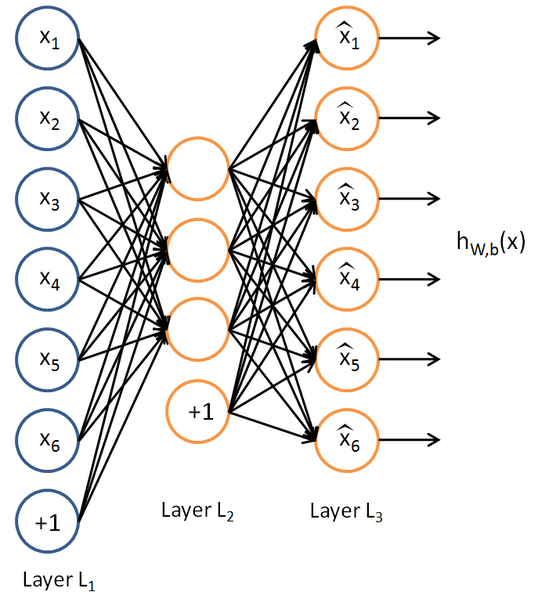
\includegraphics[width=0.9\textwidth]{autoencoder.png}
    \caption{Autoencoder}
    \label{fig:awesome_image}
\end{figure}
\begin{figure}[H!]
    \centering
    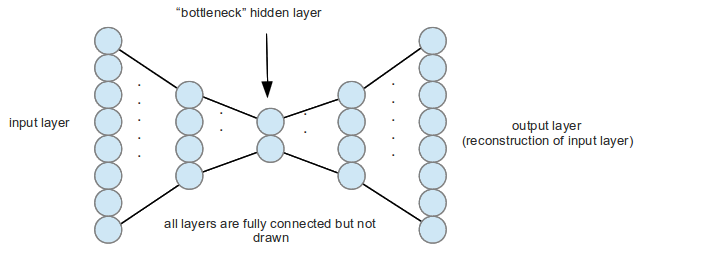
\includegraphics[width=0.9\textwidth]{stackedDAE.png}
    \caption{Stacked Autoencoder}
    \label{fig:awesome_image}
\end{figure}

\textcite{suk16} proposed that a stacked DAE can used as an intermediate building block for deeper models in neuroimaging analysis. DAE is an unsupervised multilayer feed-forward neural networks, the goal of which is setting a latent representation of feature vectors of its input by training a nonlinear approximation function $h(\textbf{f}_t) \approx \textbf{f}_t$ (Figure 1). Concretely, 
\begin{center}
$\emph{G} = \left[ \textbf{g}_1, \cdots, \textbf{g}_t, \cdots, \textbf{g}_T \right], \textbf{g}_t \in \mathbb{R}^{R}$ 
\end{center}
is expected to converted from its original form 
\begin{center}
$\emph{F} = \left[ \textbf{f}_1, \cdots, \textbf{f}_t, \cdots, \textbf{f}_T \right], \textbf{f}_t \in \mathbb{R}^{R}. $
\end{center} 

A stacked autoencoder (Figure 2) is composed of multiple layers of autoencoders, in which the outputs of each layer is fed as the inputs of successive layer \cite{stackedDAE}. Usually greedy layer-wise training is applied to train a stacked autoencoder. In current implementation, training for the stacked model is similar to the non-stacked one. Lleast-square loss function with  is selected to train the stacked model, in which the difference is directly computed between input layer and final target layer. Although that setting of the hidden layer configure is  heuristic, the combination in \textcite{suk16}'s paper is followed. 

After training, only the first part of the DAE (i.e. from input layer to bottleneck hidden layer) is used to transform each $\textbf{f}_t \in  \mathbb{R}^{R}$ into $ \textbf{x}_t \in  \mathbb{R}^{r}$, where $ r < R$. As a result, the encoded representation of a scan becomes
\begin{center}
$\emph{X} = \left[ \textbf{x}_1, \cdots, \textbf{x}_t, \cdots, \textbf{x}_T \right]$ 
\end{center}
to fed into the classification model to come. 

\subsection{High-level RNN classifiers and their ensemble for subject diagnosis}

\textcite{wee15} proposed a framework for brain functional connectivity analysis, in which each time series of each scan are decomposed into multiple overlapping sub-series by a sliding window. Justified by their work, a encoded time-series is splitted into identical-sized sub-series
\begin{center}
$\emph{X} = \left[ \textbf{x}_1, \cdots, \textbf{x}_s, \cdots, \textbf{x}_{S} \right]$, where $T=n*S, n$ is an integer. 
\end{center}
A RNN is a specialized class of neural network that is suitable for dynamic temporal sequences. Connections between units in a RNN form a directed cycle. For each unit, hidden nodes are created as internal memory to process sequences of inputs, which enables RNN to condition the model on all previous units in a sequence (Figure 3). Below are the formulas in the network.

\begin{center}
$S_k = \sigma(W^{(rec)}S_{k-1} + W^{x}x_k )$
\end{center} 
\begin{center}
$y = softmax(W^{(s)}S_k)$
\end{center}

The detailed notation is explained below:
\begin{easylist}
\ListProperties(Hide=100, Hang=true, Progressive=3ex, Style*=-- )
@ $ \textbf{x}_k \in  \mathbb{R}^{r}, k=1, \cdots , n$: the input of a unit
@ $S_k $: current hidden state
@ $W^{(rec)}$: weights matrix used to condition the hidden state of the previous time-step 
@ $W^{x}$: weights matrix used to condition the input of a unit $ \textbf{x}_k$
@ $\sigma()$: the non-linearty function ()
@ $y$: predicted class for the sequence
@ $W^{(s)}$: weight matrix that transform $S_k$ to $y$
\end{easylist}

\begin{figure}[H!]
    \centering
    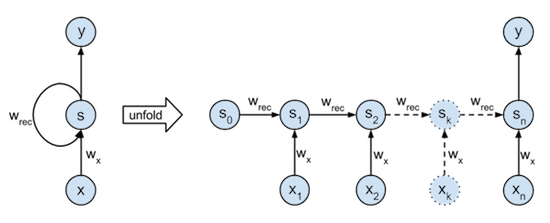
\includegraphics[width=0.9\textwidth]{rnn.png}
    \caption{Recurrent Neural Networks}
    \label{fig:awesome_image}
\end{figure}

In terms of the sub-series setting, data in each time point of a series $\textbf{x}_t$ become the input of a unit. The final output at the end of the sequence is the predicted class (AD or NC) for the whole sub-series. For the purpose of diagnosis of a subject, ensemble learning is used to predict the class for the time-series of a scan. Each high-level classifier votes with equal weight and the class with the most votes is selected as the class of a time series.


\section{Study 1}

%This study is designed as a pilot study and serves to identify the appropriate difficulty for the Petri net material.
%The amount of places and transitions and their interconnection should make the task feasible, meaning the recall rate should be far above a randomly drawn new Petri net, but still each recalled drawing should contain some error.
%Successful analyses have been conducted with accuracy measure from 58\% correct recall \cite{egan1979chunking} up to 95\% \cite{moss2006role} which is hence taken as the desired lower and upper boundary respectively.
%
%\subsection{Method}
%
%\subsubsection{Participants}
%Three first-year students, three third-year students who have taken at least one Petri net class and three scientific employees who work with Petri net related material on a daily basis shall participate in this study.
%The students' participation in experiments is mandatory and part of their curriculum, the scientific assistants get cookies as a reward.
%
%\subsubsection{Materials}
%Petri nets are randomly generated (cf. Appendix~\ref{app:generated}) and visually formatted (cf. Appendix~\ref{app:formatted}).
%A range of 5 and 30 graph elements ($n$) is used with a number of interconnections ($f$) between $f=n-1$ and $f=round(3/2 * n)$.
%Grid lines are drawn onto the background so that each place or transition is on an intersection of one of the vertical and horizontal lines.
%
%\subsubsection{Procedure}
%In the beginning the participant is introduced in using \citetitle{renew} \cite{renew} as a tool for drawing Petri nets.
%Further participant is informed that any element which is not on one of the intersections between the vertical and horizontal lines is removed during the scoring process.
%Each participant does 13 runs from which the first run is discarded as a demo run.
%In that way each participant sees 13 different Petri nets.
%The participant sits in front of the screen and is presented one of the generated Petri nets for 5 seconds.
%After that immediately the recall phase starts.
%Using \citetitle{renew} the participant is asked to reconstruct the previously seen net.
%On the background the same grid lines are presented and the participant is asked to position the places and transitions on the grid lines as the participant has seen it before.
%After the participant believes that everything which could be remembered has been drawn, the file is saved, printed and closed.
%The participant is then asked to indicate the used strategy on the print-out and circle which symbols were grouped together.
%
%\subsection{Scoring}
%\label{subsec:scoring}
%The scoring is inspired on a previous study on mechanical engineers \cite{moss2006role} which used an extended scoring system of \textcite{chase1973mind}.
%The scoring of each recall is done in the following manner:
%
%\begin{APAenumerate}
%	\item Each place and transition which is not drawn on the grid intersections is deleted (including the arcs which connected the deleted element with other elements).
%	\item  Each place and transition which has been omitted on the grid is added to the element omission score.
%	\item Each place and transition which appears on a wrong position on the grid is added to the element insertion error score.
%	\item Each arc which connects two previously unconnected elements is added to the arc wrong connection score.
%	\item Each arc which is omitted is added to the arc omission score.  
%	\item Each arc which points into the wrong direction is added to the arc wrong direction score.
%\end{APAenumerate}
%
%The total weighted error score for a drawing is the weighted sum of all the errors mentioned above.
%Each error score is weighted with $1$ except the arc wrong direction score which is weighted with $0.5$.
%
%\subsection{Data Analysis}
%
%For each participant and each Petri net first the error score is calculated.
%Then correct recall score is calculated as a sum of all correctly positioned elements.
%Then the ratio of the correct recall score to the sum of both the total weighted error score and the correct recall score is calculated.
%If this ratio is in the range of 58 to 95\%, it is selected as appropriate material.
%Otherwise the Petri net is discarded.
%Further the Petri nets are ranked according to their ratio and the rank list is partitioned into three proportions of similar sizes.
%The partitions are labeled with their respective difficulty level, viz. easy, medium and difficult.


\section{Study 2}

In this study the prepared material of the last study is used in a similar setup.
As a new component a distractor task is added to deteriorate the visual-spatial sketchpad \parencites(cf.)(){baddeley1986working}.
Further a second measure, the inter-response time analysis, is taken, to gain more insight into the nature of chunks.

\subsection{Method}

\subsubsection{Participants}
10 first-year students, 10 third-year students who have taken at least one Petri net class and 10 scientific employees who work with Petri net related material on a daily basis shall participate in this study.
As number of professors and teaching assistants of the University of Hamburg might not be sufficient, assistance from other universities which are also involved in Petri net research might be asked to help.
The students' participation in experiments is mandatory and part of their curriculum, the professionals get some cookies as a reward.
Having participated in study 1 excludes the participants from study 2.

\subsubsection{Materials}

\paragraph{Petri nets} The Petri nets which have been approved in study 1.

\paragraph{Distractor task} An unsolvable 15-puzzle \parencites(cf.)(){ratner1986finding} which runs as a program on the same computer 

\subsubsection{Procedure}
In the beginning the participant is introduced in using \citetitle{renew} \cite{renew} as a tool for drawing Petri nets.
Further the participant is informed that any element which is not on one of the intersections between the vertical and horizontal lines is removed during the scoring process.
Each participant does 13 runs from which the first run is discarded as a demo run.
The pool of Petri nets for one participant contains 6 drawings connected with the distractor -- no distractor condition.
In the no-distractor condition the net will be shown immediately whereas in the distractor condition between the presentation and the recall a 30s delay happens.
The six drawings shown in both conditions equal 12 runs.

For each run the Petri net and its connected condition is drawn randomly from the pool.
The participant sits in front of the screen and is presented the drawn Petri net for 5 seconds.
Depending on the drawn condition either the distractor task is shown or the recall starts immediately.
Using \citetitle{renew} the participant is asked to reconstruct the previously seen net.
Mouse clicks and the screen are recorded throughout the process.
On the background the same grid lines are presented and the participant is asked to position the places and transitions on the grid lines as the participant has seen it before.
After the participant believes that everything which could be remembered has been drawn, the file is saved, printed and closed.
The participant is then asked to indicate the used strategy on the print-out and circle which symbols were grouped together.

\subsection{Data Analysis}

\subsubsection{Performance Analysis}

First the error scores are calculated as described in \textit{scoring} of study 1.
A mixed-design analysis of variance (ANOVA) with 
the Petri net difficulty level (simple, medium, difficult),
the distractor task and
the total weighted error score
as a within-subjects factor and 
expertise level
as the between-subjects factor is conducted.
As a post-hoc test Tukey's HSD is chosen.
Significant differences are expected between the three groups and between the three Petri net difficulty levels.
First-year students are expected to show significant differences between the distractor task and the no distractor task condition while scientific employees are expected not to have a significant difference.

\subsubsection{Inter-Response Time Analysis}
The mouse clicks and screen recordings are analyzed using a single-linkage hierarchical clustering algorithm \parencites(cf.)(){moss2006role}.
The found chunks are supposed to correspond to the units indicated by the respective participant.
Since each drawing was both presented in the distractor and no distractor condition, for the same drawing for each participant two hierarchical clusters exist.
They are compared using the correlation between the cophenetics of each hierarchical cluster \parencites(cf.)(){fowlkes1983method}.
The two cophenetics are expected to strongly correlate for scientific employees since their are expected to be unaffected by the distractor condition whereas a rather low correlation between the two cophenetics is expected for first-year students. 
In the no distractor condition first-year students are expected to have rather complex (probably both nested and overlapping) chunks in working memory which help to recall the drawing with comparably little error.
In the distractor condition first-year students need to rely on incidental encoding to their long-term working memory.
Maybe the presented drawing can utilize existing knowledge about superficially similar visual languages like flow chart diagrams or other, probably highly personal, mnemonic strategies.
Without making elaborated assumptions about the used strategies, they are supposed to result in a different cluster than in the immediate recall condition.


\section{Implementation of this Project}




\section{Conclusion}

In this project, a new model is proposed to classify subjects with AD and NC subjects. Specially, we devise a hybrid architecture by involving RNN into the final decision process. To overcome the constraints of limited data, the high dimensional data output by the previous step is splitted into multiple identical-sized segments. We evaluates the performance of the proposed and analyzed several influential tuning decisions. As part of our future work, we hope to substitute the overlapping sliding window for identical-sized segments to further improve the performance of our model.

%\documentclass{report}
%\usepackage[verbose]{placeins}
%\usepackage[ngerman]{babel}
%\usepackage{blindtext}
% 
%\begin{document}
% 
% 
%\section{A}
%\blindtext \blindtext \blindtext
% 
%\begin{figure}[htb]\centering
%\fbox{\parbox{5cm}{\centering Bild\\[5cm]}}
%\caption{Ein Bild}
%\end{figure}
% 
%\FloatBarrier
% 
%\section{B}
% 
%\blindtext
% 
%\end{document}



\printbibliography

\appendix

\section{Visual vocabulary of an Elementary System Net}
\label{app:elsysnet}

\begin{figure}
    
\includegraphics[scale=1]{graphics/visual_vocabulary_elementary_system_net}
    \caption{A circle depicts a place, a rectangle depicts a transition and an arrow depicts and arc. The arrow connects places with transitions and can be bent for that purpose. The green color is the standard color of the }
    \label{fig:visual_vocabulary_elementary_system_net}
\end{figure}

\section{Random Petri Net Generation Algorithm}
\label{app:generated}

\begin{verbatim}
Input
  n: number of graph elements
  f: number of interconnections  
Output
  P: set of places
  T: set of transitions
  F: set of f el P x T U T x P

Algorithm
  tmp := gaussian(location=n)
  while tmp < 0:
    tmp := gaussian(location=n)
  sizeP := n - tmp
  sizeT := n - sizeP
  P := {p_1, p_2,..., p_sizeP}
  T := {t_1, t_2,..., t_sizeT}
  
  P_2 = {}
  T_2 = {}
  p_last := random element from P
  t_last := random element from T
  while f > 0:
    p_Pool := P \ P_2 if (P \ P_2) != {} else P
    t_Pool := T \ T_2 if (T \ T_2) != {} else T
    p := random(p_alt, random element from p_Pool)
    t := random(t_alt, random element from t_Pool)
    P_2 := P_2 U p
    T_2 := T_2 U t
    if random(TRUE, FALSE):
      F := F U (p, t)
      p_last := random element from P_2
      t_last := t
    else:
      F := F U (t, p)
      p_last := p
      t_last := random element from T_2
    f--
    if places or transitions are not yet connected:
      discard Petri net
\end{verbatim}

\section{Layout Algorithm}
\label{app:formatted}

\begin{verbatim}
Input
  P: set of places
  T: set of transitions
  F: set of f el P x T U T x P
Output
  Layout
  
Algorithm
  Draw grid
  Search for whether there is p el P with no incoming arc
  If yes: P_2 := all p el P with no incoming arc
  Else: P_2 := {random p el P}
  i := 0
  while F_2 != F:
    draw all p el P_2 on the ith grid line vertically arranged if not yet present 
    draw all t for which (p, t) el F on the (i+1)th grid line if not yet present
    draw the arcs between p and t for all drawn t if not yet present
    P_2 := {p | (t, p) el F for all drawn t}
    F_2 := F_2 U (t, p) U (t, p) for t, p part of the drawing
    i++
\end{verbatim}

\end{document}
